\documentclass[handout, 11pt]{beamer}
\mode
<presentation>{\usetheme{Madrid}}
\institute[UF]{\inst{1}
University of Florida\\
Department of Finance, Insurance, and Real Estate}
\usepackage{xcolor}
\usepackage{adjustbox}
\usepackage{tikz}
\definecolor{darkgreen}{RGB}{31,156,17}
\setbeamertemplate{headline}{\begin{beamercolorbox}[ht=2.25ex, dp=3.75ex]{section in head/foot}
\insertnavigation{\paperwidth}
\end{beamercolorbox}}
\AtBeginSection{\begin{frame}
\frametitle{Table of Contents}
\tableofcontents[currentsection]
\end{frame}}
\begin{document}
\title[TVM Deep Dive Python]{The Depth of a Financial Model, Continued}
\subtitle{Extending a Simple Retirement Model in Python}
\author[DeRobertis]{Nick DeRobertis\inst{1}}
\date{\today}
\begin{frame}
\titlepage
\label{title-frame}
\end{frame}
\begin{section}[Model Structure]{Structuring a Model in Python and Jupyter}
\begin{frame}
\frametitle{How to Structure a Python Financial Model}
\begin{itemize}
\item We have seen how structure and organization can help the readability and maintainability of an Excel model. The same concept exists for our Python models.
\vfill
\item We already learned that we should use functions to organize logic and a
\texttt{dataclass}
for the model inputs
\vfill
\item Typically you'll have functions for each step, those may be wrapped up into other functions which perform larger steps, and ultimately you'll have one function which does everything by calling theother functions.
\vfill
\item Those are good ideas with any Python model, but working in Jupyter allows us some additional organization and presentation of the model
\end{itemize}
\end{frame}
\begin{frame}
\frametitle{Using Jupyter for Structure of a Model}
\begin{itemize}
\item In Jupyter, we can have code, nicely formatted text, equations, sections, hyperlinks, and graphics, all in one document
\vfill
\item For all you can do with these nicely formatted "Markdown" cells, see
\textcolor{blue}{\underline{\href{https://www.markdownguide.org/basic-syntax/}{here}}}
and
\textcolor{blue}{\underline{\href{https://www.markdownguide.org/extended-syntax/}{here.}}}
\vfill
\item We can think of sections in Jupyter as analagous to Excel sheets/tabs. One section for each logical part of your model. Then you can have smaller headings for subsections of the model.
\vfill
\item Break your code up into small sections dealing with each step, with nicely formatted text explaining it. Add comments where anything is unclear in the code.
\end{itemize}
\end{frame}
\begin{frame}
\frametitle{Workflow and Final Output}
\begin{itemize}
\item When I develop in Jupyter, I have lots of cells going everywhere testing things out
\vfill
\item When I finish a project in Jupyter, I remove these testing cells and make sure it runs and logically flows from end to end
\texttt{(restart kernel and run all cells)}
\vfill
\item Run your model with different inputs, and make sure the outputs change in the expected fashion. This is a good way to check your work.
\vfill
\item There may be outputs in each section, but the final output should be at the end of the notebook
\end{itemize}
\end{frame}
\end{section}
\begin{section}[Project 1]{Project 1 Additional Material}
\begin{frame}
\frametitle{Introducing Project 1}
\begin{itemize}
\item The first project is aimed at approaching a new time value of money and cash flow model
\vfill
\item It covers the same concepts as the retirement model, but in a capital budgeting setting
\vfill
\item We need to introduce some economic equations to handle this model. You should have covered these in microeconomics.
\end{itemize}
\end{frame}
\begin{frame}
\frametitle{A Quick Review of Supply and Demand}
\begin{center}
\begin{adjustbox}{width=0.9\textwidth, height=0.8\textheight, keepaspectratio}
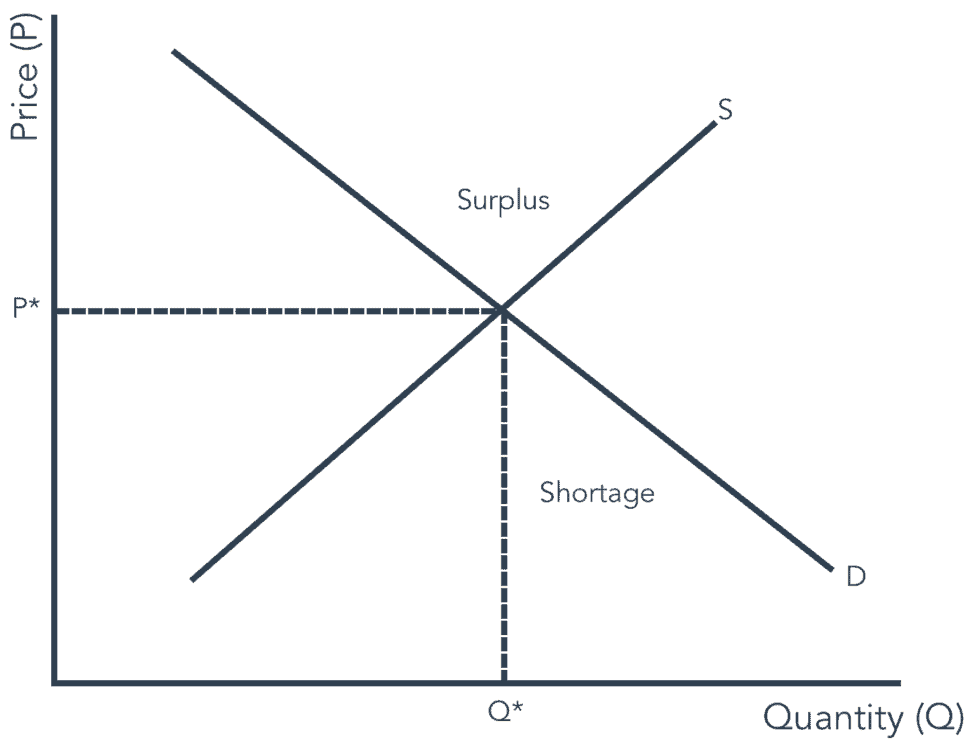
\includegraphics[width=1.0\textwidth]{Sources/supply-demand-graph.png}
\end{adjustbox}
\end{center}
\end{frame}
\begin{frame}
\frametitle{Equations for Project 1}
\begin{block}{New Required Equations}
There are a couple of basic economic equations we haven't talked about that we'll need for this:
\begin{equation}
	R = PQ
\end{equation}
\begin{equation}
	Q = min(D, S)
\end{equation}
\begin{itemize}
\item $R$: Revenue
\item $Q$: Quantity Purchased
\item $D$: Quantity Demanded
\item $S$: Quantity Supplied
\end{itemize}
\end{block}
\end{frame}
\begin{frame}
\frametitle{A Couple More Things on the Python Side}
\begin{itemize}
\item We need to cover one more Python concept and one gotcha before you can complete the first project.
\vfill
\item On the next slide I'll introduce error handling, and show an example of how it's useful
\end{itemize}
\begin{alertblock}<+>{NPV Gotcha}
\begin{itemize}
\item The NPV function in \texttt{numpy} works slightly differently than the NPV function in Excel.
\item Excel treats the first cash flow as period 1, while \texttt{numpy} treats the first cash flow as period 0.
\item If taking NPV where the first cash flow is period 1, pass directly to Excel, and for Python, pass 0 as the first cash flow, then the rest.
\item If taking NPV where the first cash flow is period 0, pass from period 1 to end to Excel and add period 0 separately, pass directly to Python.
\end{itemize}
\end{alertblock}
\end{frame}
\end{section}
\begin{section}[Build the Model]{Building the Dynamic Salary Retirement Model}
\definecolor{darkgreen}{RGB}{15,82,13}
\begin{frame}
\frametitle{The Structure of the Retirement Model}
\begin{center}
\begin{adjustbox}{width=0.9\textwidth, height=0.8\textheight, keepaspectratio}
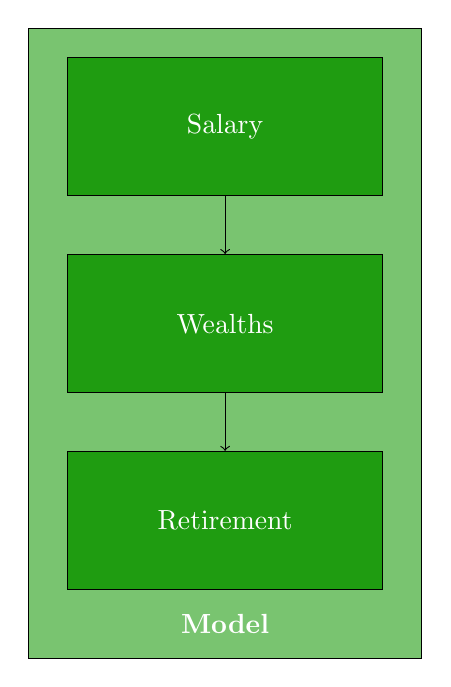
\begin{tikzpicture}
\coordinate [fill=darkgreen!60, minimum width=5cm, minimum height=8cm, rectangle, draw] (c76dabc2-1964-4a10-b72a-88fafa6f2138) at (1.25, 4) {};
\node [text=white, above=0.2cm ] (ab3d5dad-7dfb-43ae-aa5d-3acc752e0aad) at (c76dabc2-1964-4a10-b72a-88fafa6f2138.south) {\textbf{Model}};
\node [fill=darkgreen, minimum width=4cm, minimum height=1.75cm, rectangle, draw, text=white] (f9bf7c24-76fd-46b5-aab1-e33305c3d589) at (1.25, 6.75) {Salary};
\node [fill=darkgreen, minimum width=4cm, minimum height=1.75cm, rectangle, draw, text=white] (77b7cfc5-f237-4b8b-ade6-b2b41b402949) at (1.25, 4.25) {Wealths};
\node [fill=darkgreen, minimum width=4cm, minimum height=1.75cm, rectangle, draw, text=white] (170050d0-04a2-4a41-8a84-c7c58c1e31e8) at (1.25, 1.75) {Retirement};
\path [draw, ->] (f9bf7c24-76fd-46b5-aab1-e33305c3d589) -- (77b7cfc5-f237-4b8b-ade6-b2b41b402949);
\path [draw, ->] (77b7cfc5-f237-4b8b-ade6-b2b41b402949) -- (170050d0-04a2-4a41-8a84-c7c58c1e31e8);
\end{tikzpicture}
\end{adjustbox}
\end{center}
\end{frame}
\begin{frame}
\frametitle{Revisiting the Model Salary Equation}
\begin{block}{Salary with Promotions and Cost of Living Raises}
\begin{center}
\begin{adjustbox}{width=0.9\textwidth, height=0.8\textheight, keepaspectratio}
$S_t = S_0 (1 + r_l)^t (1 + r_p)^p$
\end{adjustbox}
\end{center}
\begin{itemize}
\item $S_t$:  Salary at year $t$
\item $S_0$:  Starting wealth
\item $r_l$:  Return for cost of living
\item $r_p$:  Return for promotion
\item $t$:  Number of years
\item $p$:  Number of promotions
\end{itemize}
\end{block}
\end{frame}
\begin{frame}
\frametitle{Building the Wealth Model}
\begin{itemize}[<+->]
\item For wealths, we need to add the investment return and then the savings in each year
\end{itemize}
\vfill
\begin{block}<+->{Calculating Wealth}
\begin{center}
\begin{adjustbox}{width=0.9\textwidth, height=0.8\textheight, keepaspectratio}
$W_t = W_{t-1}  (1 + r_i) + S_t  v$
\end{adjustbox}
\end{center}
\begin{itemize}
\item $S_t$:  Salary at year $t$
\item $W_t$:  Wealth at year $t$
\item $r_i$:  Investment return
\item $t$:  Number of years
\item $v$:  Savings rate
\end{itemize}
\end{block}
\end{frame}
\begin{frame}
\frametitle{Creating a Full Model in Python}
{
\setbeamercolor{block title}{bg=darkgreen}
\begin{block}{Dynamic Salary Retirement Model in Python}
\begin{itemize}
\item I will now show the process I use to create a full model.
\item I will be recreating the model in Examples > Intro > Python > Dynamic Salary Retirement Model.ipynb
\item Go ahead and download that to follow along as you will also extend it in a lab exercise
\end{itemize}
\end{block}
}
\end{frame}
\begin{frame}
\frametitle{Relaxing the Static Desired Cash in Python}
\begin{itemize}
\item We want to relax the assumption that the amount needed in retirement is given by a fixed amount of desired cash
\end{itemize}
\vfill
{
\setbeamercolor{block title}{bg=violet}
\begin{block}{Modeling Desired Cash}
\begin{itemize}
\item Start from the completed retirement model Dynamic Salary Retirement Model.ipynb 
\item Add new inputs to the model, "Annual Cash Spend During Retirement" and "Years in Retirement"
\item Calculate desired cash based on interest, cash spend, and years in retirement
\item Use the calculated desired cash in the model to determine years to retirement
\item If annual spend is 40k for 25 years in retirement, \$563,757.78 should be the retirement cash
\end{itemize}
\vfill
\end{block}
}
\end{frame}
\begin{frame}
\frametitle{Extending the Simple Retirement Model in a Different Way, Level 1}
{
\setbeamercolor{block title}{bg=violet}
\begin{block}{Practice Building A Model, Level 1}
\begin{enumerate}
\item Usually I would try to have smaller labs but it didn't fit the format of this lecture. Most will not be able to complete this during class.
\item For this lab, attempt the practice problem in Practice > Retirement > P1 Python Retirement Savings Rate Problem.pdf
\item This is similar to how the projects will be assigned, so it is good preparation
\item I would encourage you to try it from scratch. If you are totally stuck, try working off of the retirement model I completed today to have a lot of the structure already. If you still are having trouble with that, check the solution and see me in office hours.
\end{enumerate}
\vfill
\end{block}
}
\label{lab:retire-model-1}
\end{frame}
\begin{frame}
\frametitle{Some Time to Work on the First Project}
{
\setbeamercolor{block title}{bg=violet}
\begin{block}{Project 1}
\begin{itemize}
\item Download and open the Project 1 document from Canvas
\item It is up to you whether you want to attempt the Excel or Python model first
\item If you feel comfortable with the Excel model, you may want to start with Python so I can give help on that today.
\end{itemize}
\vfill
\end{block}
}
\end{frame}
\end{section}
\end{document}